
\newpage 
\section{An Introduction to Programming}

\subsection{Designing computer programs}

Designing a computer program is a complicated business. It requires a 
great deal of creativity, a considerable understanding of the task or process
being automated, a good eye for accuracy, and finally a large degree of 
patience. 

In industry, the process of designing a computer program is separated from
the task of actually writing the program itself. This is because the skills
required for each task can be quite different. 

The process of program design often starts with an idea supplied by a 
{\em customer}. The customer may telephone you stating that they are 
considering automating a shampoo bottling plant, and that they need a program
to control the machinery. The program designer's task is then to write 
a document stating exactly what the 
customer requires, which can then be passed on to the programmers
and turned into code; this document is called the {\em program specification}. 

Writing a program specification is difficult, particularly because you 
need to pitch it at exactly the right level. A specification which states 

\begin{quote}
``Get some bottles, put some shampoo in and then put them in the boxes''
\end{quote}

is probably not detailed enough for a programmer to successfully write a 
piece of code which will do exactly what the customer is looking for. The
programmer may (legitimately) write some code which gets 2000 bottles at a
time for example; this after all meets the specification, though probably does not 
fit with the machinery available. 

Alternatively, a specification which states

\begin{quote}
Line 10: Assign to the first variable the result of -- If the first bottle is
ready and there is some shampoo in the machine or the green light is on
then ...
\end{quote}

may be too detailed for the programmer to have complete control over the 
implementation. The specification will probably also be extremely long and 
may, as here, contain ambiguities. 

So as you can see, writing a specification is not as straightforward as it 
first seems. 

\begin{figure}
\centering
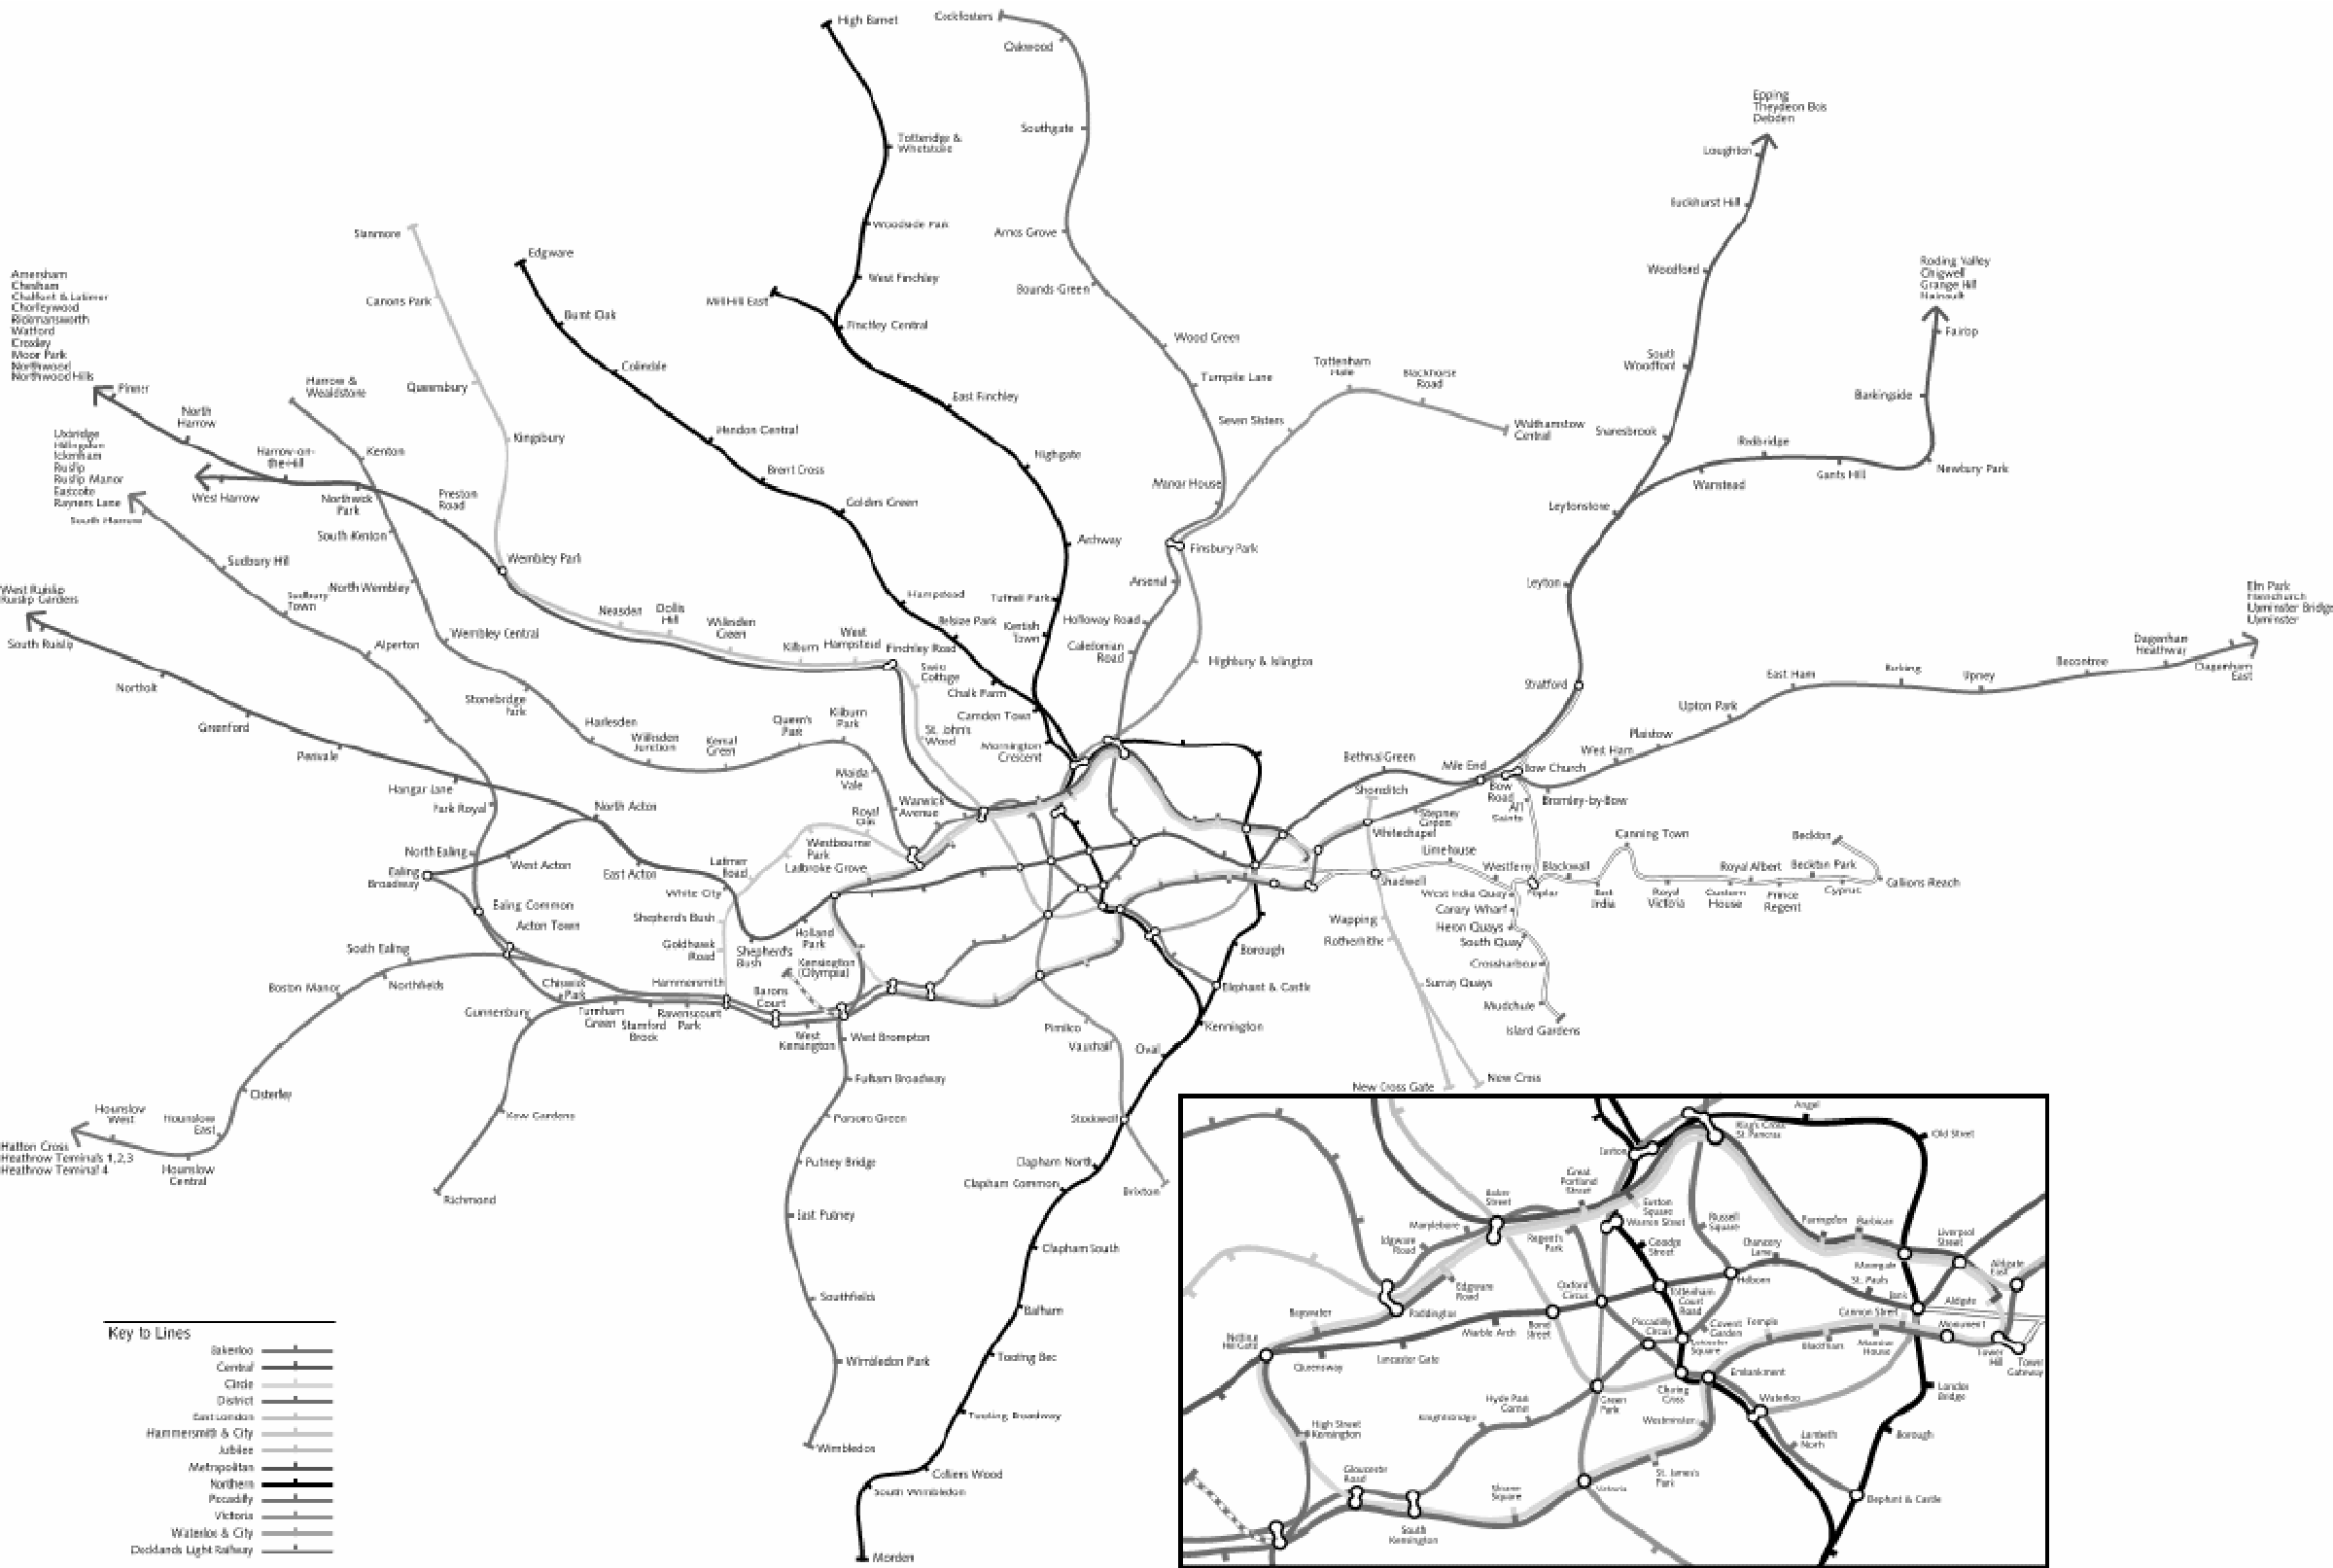
\includegraphics[width=5in]{geog}
\caption{\small The geographical representation of the London
                underground\label{train1}}
\end{figure}


\subsubsection{The Diagram}

Consider the following example based on that found in the excellent book 
{\em Using Z:
Specification, Refinement and Proof} by Jim Woodcock and Jim Davies:  \\

\noindent
Writing a specification at an appropriate level of abstraction is essential. 
A good example of this is provided by the various maps of the London 
Underground. When the first map was published in 1908, it was faithful to the 
geography of the lines: the shape of the track and distance between stations 
were faithfully recorded. However, the purpose of the map was to show 
travellers the order of stations on each line, and the various interchanges
between lines; the fidelity of the map made it difficult to extract this 
information. Figure~\ref{train1} shows the geographical representation of the 
London underground. \\

\noindent
The map was changed in 1933 to a more abstract representation which was 
rather nicely named \emph{The Diagram}. 
The draughtsman Harry Beck, who produced the imaginative yet stunningly 
simple design, based the map on the circuit diagrams he drew for his day 
job. All the detail concerning connectivity
was maintained, though the simplification meant that passengers could 
see at a glance the route to their destination. Abstraction from 
superfluous detail -- in this case the physical layout of the lines -- was 
the key to the usefulness of The Diagram. The Diagram 
can be seen in Figure~\ref{train2}. \\



\begin{figure}
\centering
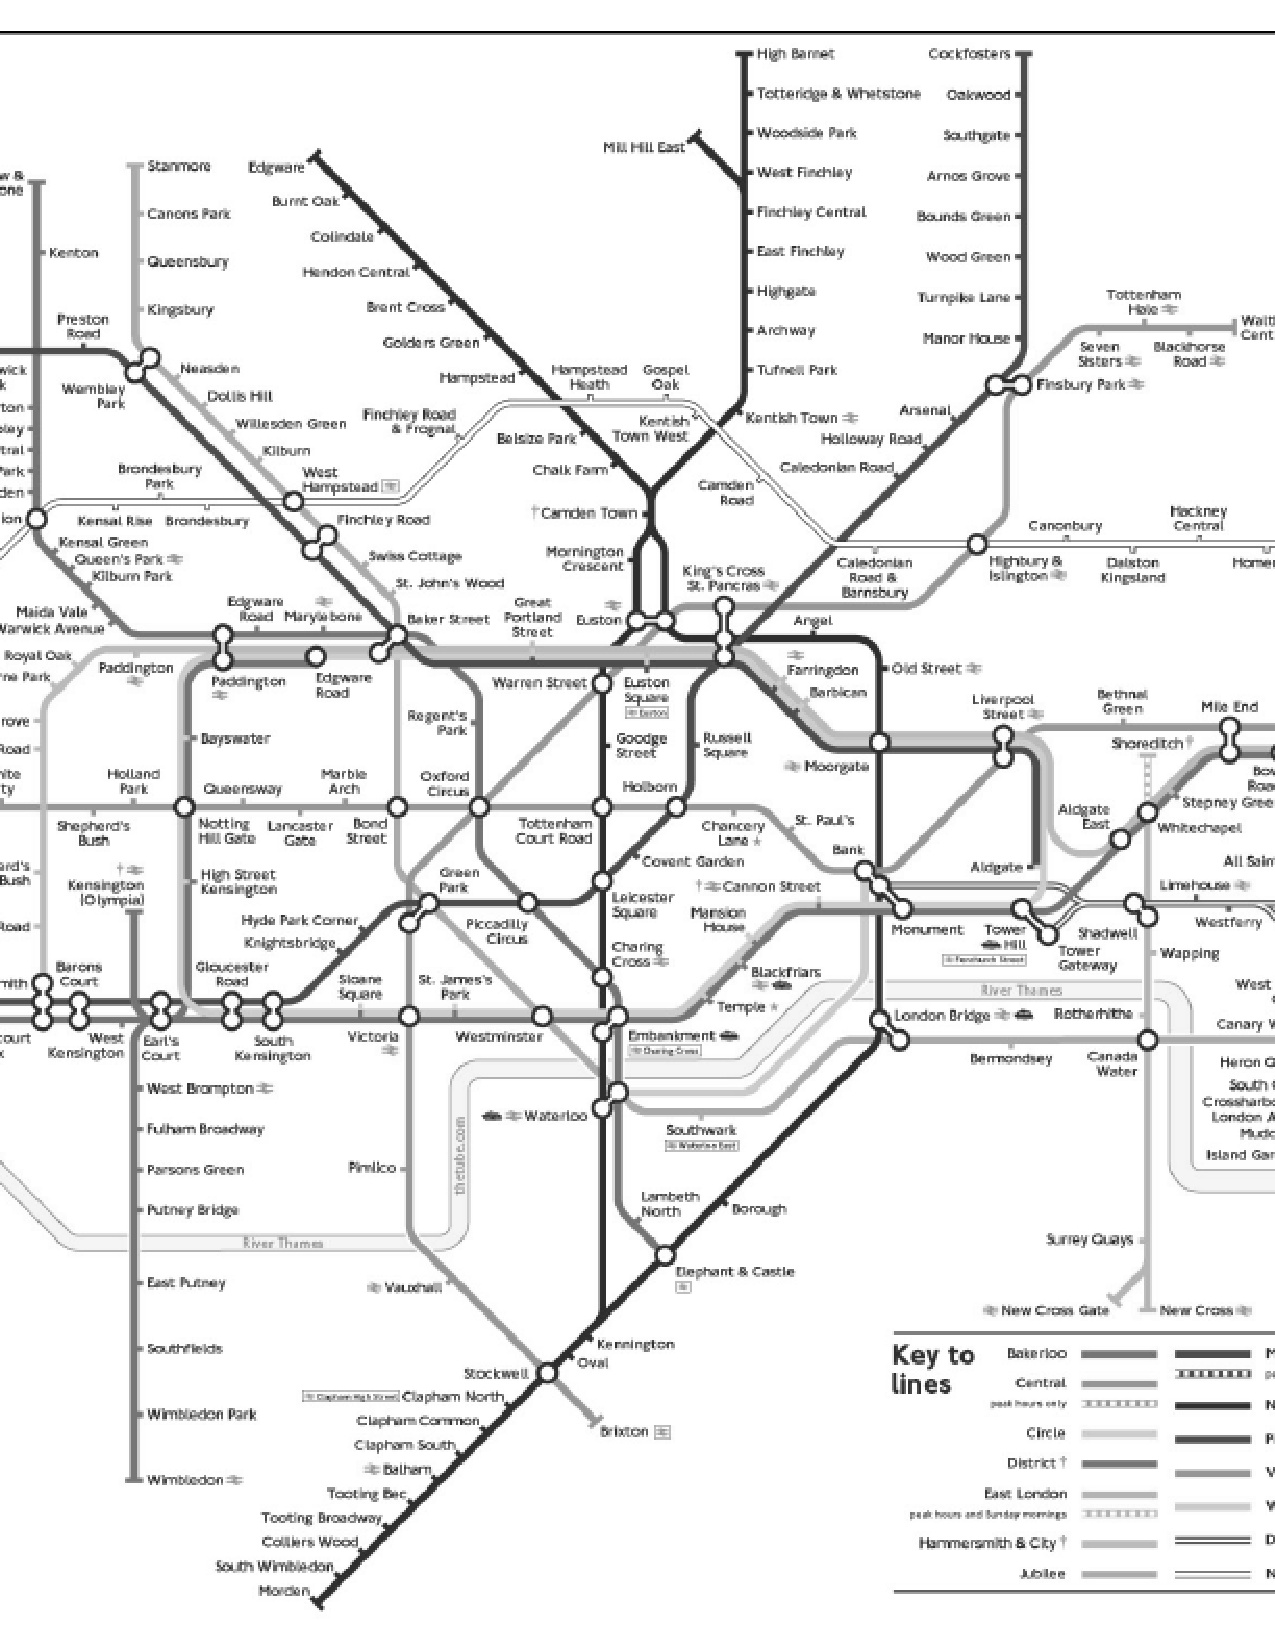
\includegraphics[width=5in]{tube_map}
  \caption{\small The Diagram, 1933; a more abstract description 
           \label{train2}}
\end{figure}

The Diagram was, and still is, a good specification of the London 
Underground. It is 

\begin{itemize}
\item
{\em Abstract}. Since it only records logical layout, not the physical 
reality in all its detail.

\item
{\em Concise}. Since it is printed on a single A5 piece of paper which is 
folded in such a way that it fits exactly into your pocket. 

\item
{\em Complete}. As every station on the London Underground network is 
represented.

\item
{\em Unambiguous}. Since the meaning of the symbols used is explained, and
the Diagram is represented in simple geometric terms. 

\item
{\em Maintainable}. Since it has been successfully maintained over the last
60 years, reflecting the changes to the network as new stations and lines 
have been opened and others have been closed. 

\item
{\em Comprehensible}. It must be readily understood by the general public. 
This has been the case as it has been regarded fondly by its users since 
1933. 

\item
{\em Cost-effective}. Since it only cost five guineas to commission the
specification from the engineering draughtsman Harry Beck. 
\end{itemize}

The Diagram gives its users a good conceptual model. It embodies a specification
structure that enables users to make sense out of a rather complex implementation. 
To do this it uses abstract shapes, colours and compression. All lines
are reduced to ninety or forty-five degree angles and the central area, 
where there are more stations, is shown in greater detail than the outlying 
parts, as if The Diagram were viewed through a convex lens. \\

The Diagram is an excellent example of a specification. You may be 
interested to know that it was first rejected by the Publicity Department of 
the London Underground, as the abstract notation was thought to be too strange
and incomprehensible for the ordinary user of the Underground network. 

\subsubsection{Writing your own specifications} 

Of course not all specifications can be dealt with in a nice pictorial form
such as The Diagram. Most specifications in fact use {\em Natural Language} and/or
some form of {\em Mathematics} or {\em Logic}. \\

Natural Language is perhaps the easiest way to communicate ideas, as most of 
us understand one language or another, English or Spanish for example. If you are to 
write specifications in a natural language then you must make sure that the
specification is unambiguous. The specification for a shampoo bottling firm
was unclear.

\begin{quote}
Line 10: Assign to the first variable the result of -- If the first bottle is
ready and there is some shampoo in the machine or the green light is on
then ...
\end{quote}

\noindent
We cannot be sure whether the `or' goes with the `shampoo
in the machine' part of the sentence, or with the 
`If the first bottle is ready and there is some shampoo in the machine' part 
of the sentence. \\

\noindent
We might make more sense of the definition by adding some mathematical notation
(brackets in this case),

\begin{quote}
Line 10: Assign to the first variable the result of -- (If the first bottle is
ready and there is some shampoo in the machine) or (the green light is on)
then ...
\end{quote}

\noindent
or by employing some logic

\begin{quote}
A = First bottle is ready \\
B = Shampoo is in the machine \\
C = Green light is on \\ 

Line 10: Assign to the first variable the result of -- ((A $\land$ B) $\lor$ C)
\end{quote}

\noindent
This final example uses some {\em Propositional logic}; three propositions are
defined (A, B and C) and they are combined using the logical 
AND ($\land$) and OR ($\lor$)
operators. The advantage that we see here is that the closer we move towards 
maths (or logic) the less chance there is of introducing any ambiguities. 

\subsection{Building computer programs}

Building a computer program is the task traditionally described
as {\em programming}. \\

\noindent
Despite many misconceptions, programming is not about sitting at a
desk full of cans of red bull and bashing out some obscure lines of text
which resemble the programmer's thoughts on a particular problem. Programming
is an exact and detailed science which involves translating {\em abstract} 
specifications
into more {\em concrete} implementations. The concrete implementation
is traditionally known as program {\em code}. 

\subsubsection{Abstract and concrete}

So what exactly is all this talk about {\em concrete} and {\em abstract}?\\

\noindent
You have seen already, in the description of a specification, that when we 
describe a problem which we may want to computerise, we should choose 
carefully the level of detail at which the problem is described. 
In writing a specification 
we must not get drawn in to any nitty-gritty points which are not
wholly in the domain of the problem itself. But why do we make such a
fuss about this, and does it really matter?\\

\noindent
Well, yes it does. When we program it is desirable to have as much freedom as 
possible: the freedom to choose a suitable programming language; choose 
our own structure and individual style; and maybe reuse bits of programs, 
to save time or money for example.  \\

\begin{figure}
\centering
\includegraphics[width=5in]{abstract.pdf}
  \caption{\small Example of abstract- and concrete-level design 
           \label{specimp}}
\end{figure}

\noindent
In fact, it is possible to have many different programs 
which implement the same specification. Consider Figure~\ref{specimp} for example.
Here we have a specification which states, ``Choose a number between 1 and 
100''. There are three implementations of this specification in the figure: 

\begin{itemize}

\item
The first program simply produces the number 10. This, you may think, does
not meet the specification given, but think about it carefully. The 
specification says choose a number between 1 and 100, and the program does,
it chooses the number 10. It chooses the number 10 each time the
program is run of course, which 
is probably not what the person who wrote the specification wanted to happen.
But the specification does not say that the number chosen should be different
each time the program is run, so effectively the program is a perfectly 
good implementation of the specification. 

\item
The second program produces a random number between 10 and 30. This also 
meets the specification as the program certainly does choose a number 
between 1 and 100. Again, this is probably not what the person who wrote
the specification intended. 

\item
The third program is probably what you would have expected. It randomly chooses
a number 
between 1 and 100. This also meets the specification and had the 
specification been written more carefully, stating, ``...a different number
in this range should be chosen with equal chance each time the program is 
run...'', then this would be the only valid implementation of the 
specification written above.

\end{itemize}

\noindent
This may seem a little confusing. Why is it useful to have a number of 
possible computer programs which implement a single abstract specification?
The point is
that it may not matter to the customer exactly what the program does,  
provided that it is within the bounds of the specification. Therefore, the 
programmer has flexibility when producing a program, and the customer
receives a program which meets their requirements. Everyone wins. \\

\noindent
Abstract specifications are useful as they allow customers who might
be ordering a computer system to write a collection of unambiguous
requirements. They may pass this specification to a number of different
programmers and receive a number of different programs
back. Although these programs may be different and may be written in a
number of different programming languages, on a number of different
machines, they will all act
exactly as the specification states. The specification therefore acts
as a {\em contract} between the customer and the programmer, and a
contract between the abstract description and the concrete
implementation. 


\subsubsection{Translation}

Programming is the business of taking an abstract-level specification
and translating it into a concrete-level piece of code, and, as we have already seen,  programmers may
do this translation in an assortment of different ways. \\

\noindent
The translation between an abstract-level specification and a concrete-level
design is actually called {\em refinement}. Each of the programs
in Figure~\ref{specimp} is a valid refinement of the specification. \\

\noindent
Just as it is important to carefully write a specification, it is also 
important to make sure that the program implementation is an accurate
coding of the description in the specification. \\

\noindent
Usually a specification will have a number of complicated clauses, and 
may also span a number of pages. Although the specification 
may be exact in its description, a programmer may make a mistake 
when reading it and consequently code something different. For this 
reason, some specification methods have complicated mathematical rules 
which translate a piece of the specification (usually written mathematically)
into the corresponding piece of program code. These rules are 
known as {\em refinement rules}. You will learn more about these if
you choose to do the software specification course later in your degree.
 

\subsection{Testing computer programs}

Testing a computer program is an extremely important business. There are many
examples which I can cite where software has failed due to inadequate testing.
 Rather than 
bore you with a complete chronology, consider the following example:\\

\noindent
The story of Ariane 5 is a good one.
In the thrust direction control unit, 
code was reused from Ariane 4.
In this code, horizontal speed was represented
by a 16-bit value.
But horizontal speed in Ariane 5 was greater,
and caused an overflow, which raised an exception.
The specification said (very foolishly) that
if an exception arose, the processor should be 
shut down and restarted.
Shutting the processor down caused the thrust
direction to jump suddenly sideways, which
broke the rocket in half.\\

\noindent
Of course not every example of software failure will end in a disaster 
quite as catastrophic as this. However, the consequences of your code failing 
may prove to have just as much of an impact on the results of a small company,
or on the grade assigned to your computing assignment, for example. \\

\noindent
Testing is defined as the detection of failure; failure is the 
departure of the behaviour of a program from its requirements. Unfortunately,
it is not possible to show the absence of failure by testing, as testing 
will only tell us whether a program fails in a particular scenario or not.
The purpose of testing is to eliminate as many problems in the code as 
possible. This  
increases the programmer's (and user's) confidence in the piece of code. As
the number of failures detected in a program becomes less, the more you will 
feel that the program exhibits the correct behaviour.      

\subsubsection{Methods of testing}

The experimental science of software testing has been the subject of research
for a number of years. Consequently, there are a number of testing methods
which are shown to be effective. We will see, and use, a few of these methods
in this course. 

\paragraph{Test of logical paths of program} One useful way to test a program is to check all the logical
paths. Consider this example:

\begin{verbatim}
   while (x < 10) {
       if (even(x)) {
           System.out.println("The number is even\n");
        } else {
           System.out.println("The number is odd\n");
           x = x + 1;
       }
   }
\end{verbatim}

\noindent
To test the logical paths of this short piece of code the user would need 
to design tests to cover at least three cases: The case when {\tt x} is 
greater than or equal to 10, in which case the while loop would not be
executed at all; the case when {\tt x} is less than 10 and is even, in which 
case you would expect {\tt The number is even} to be printed at least once, 
and finally the test when {\tt x} is less than 10 and is odd, in which case 
you would expect {\tt The number is odd} to be printed at least once. \\

\noindent
Forgetting one of these cases will mean that you have not tested part of the 
code; this may be the piece of code which blows up, or
wipes the hard disk, or .... Would you expect any of the logical paths
in the program to reveal an error in the above code?

\paragraph{Range of inputs} Another way to test the example program would have been to test the range of 
inputs. If we can be sure that the program produces the right output for
each valid (and even invalid) input, then we can be a bit more sure that it
does what we expect. We may for example have tested the program with a 
negative value, a positive value and the value 0. \\

\noindent
Boundary cases are also important. You may want to check that the computer
deals correctly with the highest possible number and the lowest possible 
number. Finally, you may want to put some spurious values into the program --
what happens when you type in a character for example, or if you just press 
the enter key, or if you just sit on the keyboard?!\\

\noindent
Of course you have to select your range of inputs carefully. Selecting the 
numbers {\tt 137645813451875},  
{\tt 0.14643528745}, {\tt -23} and {\tt 19}, say, 
would not have found the infinite loop in the program.

\paragraph{Systematic tests} It is all very well to test the logical paths of the program and
the ranges of input, but it is sometimes the sequence of operations in
a program which causes it to break. For example, the `landing-gear down' and
`increase throttle' routines may both work exceptionally well by themselves, 
but putting the landing-gear down and then increasing the throttle may cause
the plane to head towards the ground at a rapid speed. This is probably not
what you want.  \\

\noindent
It may be worth testing a sequence of operations in your program, testing
all the permutations of the routines {\em a}, {\em b} and {\em c} for example,
to make sure that one does not exhibit any unexpected behaviour. 

\paragraph{Random tests} Random testing is a perfectly legitimate activity, but do not expect it to 
consistently come up with all the errors which may be detected by a logical or
systematic approach. \\

A true random test of a program is actually quite difficult to 
achieve. It would probably require a random number generator to 
choose between the routines in the program which were to be  
tested. A random test would also require a similar random 
selection activity to choose random input data to the program;
of course the amount of data itself must also be randomly chosen.
So be careful when you use the term `random testing'.
 
\paragraph{Intuitive tests} The process that people often think of as random testing is actually called {\it intuitive testing}. \\

After you have spent some time programming you may become aware of common
errors which appear in programs. A program which stores and deletes a 
collection of names will often be fooled if the first thing you ask it to 
do is to delete. Programs which accept characters as input will often break 
if you feed in a control character (which is a special character that cannot be printed
to screen).

Choosing cases like this to test your program is not a random 
activity -- you are usually selecting the tests based on your 
intuition as a programmer. So when you run a program for the 
first time and select a number of seemingly random operations, 
you will probably find yourself going through a number of cases
which you expect to work, followed by one or two cases in which 
you think the program may break. 

These tests usually require a bit of 
thought, but you can come up with some interesting results quite quickly. 
 

\paragraph{Test application} A {\em test application} is a piece of software which will run alongside the program to be tested. The test application may 
generate test data, supply tests, and record and calibrate the 
results as the testing takes place. Test applications are useful as they automate 
the testing process, removing any possibility of human error.
They also allow a large number of tests to be carried out 
automatically; you may for example run the test application over night, checking the 
results the following morning. \\

Test rigs also allow large systems to be tested with relative ease. Programmers
of large systems, those used by banks for example, often use test rigs 
when they are modifying the system. This means that the results before and after 
the modification can be compared to make sure that the system is still 
operating correctly. \\

One thing which is slightly ironic about test rigs is that they
themselves need testing, perhaps with test rigs, which themselves... \\

You might try some of these test methods later in the course. \\

The method of testing you use will often be dictated by a number of factors. 
You may not have time to carry out a logical or systematic test and an
intuitive test will have to do; it may be essential that you identify as many errors as 
possible, in which case random and range testing might not be good enough. It 
is up to you as a programmer to weigh up these factors to determine which 
method is appropriate given the situation. 
 
